%! TEX TS-program = lualatex
\documentclass[border=8pt, multi, tikz]{standalone} 

\usepackage{fontspec}
\usepackage{unicode-math}
\usepackage{ifthen}
\setmainfont[
	Ligatures=TeX,
	% TODO: Uncommenting the following line breaks compilation
	% TODO: I do want old style numerals, but only in the text and not in tables
	Numbers={OldStyle}, %, Proportional},
	SmallCapsFeatures={LetterSpace=3, Renderer=Basic},
]{Linux Libertine O}
\setmonofont[Scale=MatchLowercase]{DejaVu Sans Mono}
% \setmathfont[Scale=MatchUppercase]{libertinusmath-regular.otf}
\setmathfont{Asana-Math.otf}
%\ProvidesPackage{init}
\usetikzlibrary{quotes,arrows.meta}
\usetikzlibrary{positioning}


\usepackage{Ball}
\usepackage{Box}
\usepackage{RightBandedBox}


\usetikzlibrary{positioning}
\usetikzlibrary{3d} %for including external image 

\def\ConvColor{rgb:green,2;red,2;blue,2}
\def\ConvReluColor{rgb:yellow,5;red,5;white,5}
\def\PoolColor{rgb:red,1;black,0.3}
\def\UnpoolColor{rgb:blue,2;green,1;black,0.3}
\def\FcColor{rgb:blue,5;red,2.5;white,5}
\def\FcReluColor{rgb:blue,5;red,5;white,4}
\def\SoftmaxColor{rgb:magenta,5;black,7}   
\def\SumColor{rgb:blue,5;green,15}
\definecolor{convtransposecolor}{HTML}{3F4688}
\definecolor{convcolor}{HTML}{3F4688}

\newcommand{\copymidarrow}{\tikz \draw[-Stealth,line width=1.5mm,draw={rgb:blue,4;red,1;green,1;black,3}] (-0.3,0) -- ++(0.3,0);}

\def\edgecolor{rgb:blue,4;red,1;green,4;black,3}
\newcommand{\midarrow}{\tikz \draw[-Stealth,line width =1.5mm,draw=\edgecolor] (-0.3,0) -- ++(0.3,0);}
\newcommand{\midarrowT}{\tikz \draw[-Stealth,line width =1.5mm,draw=\edgecolor] (-0.3,0) -- ++(0.3,0);}
\newcommand{\midarrowFC}{\tikz \draw[-Stealth,line width =1.5mm,draw=\FcColor] (-0.3,0) -- ++(0.3,0);}
\begin{document}
\begin{tikzpicture}
\tikzstyle{connection}=[line width=3.pt,every node/.style={sloped,allow upside down},draw=\edgecolor,opacity=0.9]
\tikzstyle{connectionT}=[line width=3.pt,every node/.style={sloped,allow upside down}, dashed, draw=\edgecolor,opacity=0.9]
\tikzstyle{copyconnection}=[line width=3.pt,every node/.style={sloped,allow upside down},draw={rgb:blue,4;red,1;green,1;black,3},opacity=0.9]
\tikzstyle{copyconnectionT}=[line width=3.pt,every node/.style={sloped,allow upside down},draw=green,opacity=0.9]

\node[canvas is zy plane at x=0] (temp) at (-3,0,0) {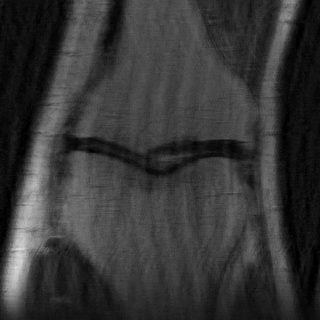
\includegraphics[width=8cm,height=8cm]{../../../regularizers/scripts/gradient/input}};

\pic[shift={(-2,0,0)}] at (0,0,0) 
    {Box={
        name=cr1,
        caption= ,
        xlabel={{48, }},
        zlabel=320,
        fill=\ConvColor,
		opacity=.2,
        height=40,
        width=1,
        depth=40
        }
    };

\pic[shift={ (1,-2,0) }] at (cr1-east) 
    {Box={
        name=ccr1,
        caption= ,
        xlabel={{ 48, 48 }},
        zlabel=160,
        fill=\ConvColor,
		opacity=.2,
        height=30,
        width={ 2 , 2 },
        depth=30
        }
    };

\draw [connection]  (cr1-east)    -- node {\midarrow} (ccr1-west);

\pic[shift={ (1,-2,0) }] at (ccr1-east) 
    {Box={
        name=ccr2,
        caption= ,
        xlabel={{ 144, 144 }},
        zlabel=80,
        fill=\ConvColor,
		opacity=.2,
        height=20,
        width={ 4 , 4 },
        depth=20
        }
    };

\draw [connection]  (ccr1-east)    -- node {\midarrow} (ccr2-west);

\pic[shift={ (1,-2,0) }] at (ccr2-east) 
    {Box={
        name=ccr3,
        caption= ,
        xlabel={{ 240, 240 }},
        zlabel=40,
        fill=\ConvColor,
		opacity=.2,
        height=10,
        width={ 7 , 7 },
        depth=10
        }
    };

\draw [connection]  (ccr2-east)    -- node {\midarrow} (ccr3-west);

\pic[shift={ (1,-2,0) }] at (ccr3-east) 
    {Box={
        name=ccr4,
        caption= ,
        xlabel={{ 432, 432 }},
        zlabel=20,
        fill=\ConvColor,
		opacity=.2,
        height=5,
        width={ 10 , 10 },
        depth=5
        }
    };

\draw [connection]  (ccr3-east)    -- node {\midarrow} (ccr4-west);

\pic[shift={ (0,-2,0) }] at (ccr4-east) 
    {Box={
        name=ccr5,
        caption= ,
        xlabel={{ 768, 768 }},
        zlabel=10,
        fill=\ConvColor,
		opacity=.2,
        height=3,
        width={ 15 , 15 },
        depth=3
        }
    };

\draw [connection]  (ccr4-east)    -- node {\midarrow} (ccr5-west);

\pic[shift={(0,-2,0)}] at (ccr5-east) 
    {Box={
        name=cr6,
        caption= ,
        xlabel={{1344, }},
        zlabel=5,
        fill=\ConvColor,
		opacity=.2,
        height=2,
		width={20},
        depth=2
        }
    };

\draw [connection]  (ccr5-east)    -- node {\midarrow} (cr6-west);

\pic[shift={(0.5,-2,0)}] at (cr6-east) 
    {Box={
        name=cr7,
        caption= ,
        xlabel={{1, }},
        zlabel=1,
        fill=\ConvColor,
		opacity=.2,
        height=1,
        width=1,
        depth=1
        }
    };

\draw [connection, draw=\FcColor]  (cr6-east)    -- node {\midarrowFC} (cr7-west);

\pic[shift={(0.5,2,0)}] at (cr7-east) 
    {Box={
        name=cr6T,
        caption= ,
        xlabel={{1344, }},
        zlabel=5,
        fill=\ConvColor,
		opacity=.2,
        height=2,
		width={20},
        depth=2
        }
    };

	\draw [connectionT, draw=\FcColor]  (cr7-east)    -- node {\midarrowFC} (cr6T-west) node [midway, below] {\( |\,\cdot\,|^\prime \)};
	\node [below of=cr7-south] {\Large \( R(\,\cdot\,,\theta) = |\,\cdot\,| \)};
	\draw [thick] (cr7-farsoutheast) to [out=-30, in=90] ++(.9, -.8);

\pic[shift={ (0,2,0) }] at (cr6T-east) 
    {Box={
        name=ccr5T,
        caption= ,
        xlabel={{ 768, 768 }},
        zlabel=10,
        fill=\ConvColor,
		opacity=.2,
        height=3,
        width={ 15 , 15 },
        depth=3
        }
    };

\draw [connectionT]  (cr6T-east)    -- node {\midarrowT} (ccr5T-west);

\pic[shift={ (0,2,0) }] at (ccr5T-east) 
    {Box={
        name=ccr4T,
        caption= ,
        xlabel={{ 432, 432 }},
        zlabel=20,
        fill=\ConvColor,
		opacity=.2,
        height=5,
        width={ 10 , 10 },
        depth=5
        }
    };

\draw [connectionT] (ccr5T-east) -- node {\midarrowT} (ccr4T-west);

\pic[shift={ (1,2,0) }] at (ccr4T-east) 
    {Box={
        name=ccr3T,
        caption= ,
        xlabel={{ 240, 240 }},
        zlabel=40,
        fill=\ConvColor,
		opacity=.2,
        height=10,
        width={ 7 , 7 },
        depth=10
        }
    };

\draw [connectionT]  (ccr4T-east)    -- node {\midarrowT} (ccr3T-west);

\pic[shift={ (1,2,0) }] at (ccr3T-east) 
    {Box={
        name=ccr2T,
        caption= ,
        xlabel={{ 144, 144 }},
        zlabel=80,
        fill=\ConvColor,
		opacity=.2,
        height=20,
        width={ 4 , 4 },
        depth=20
        }
    };

\draw [connectionT]  (ccr3T-east)    -- node {\midarrowT} (ccr2T-west);

\pic[shift={ (1.3,2,0) }] at (ccr2T-east) 
    {Box={
        name=ccr1T,
        caption= ,
        xlabel={{ 48, 48 }},
        zlabel=160,
        fill=\ConvColor,
		opacity=.2,
        height=30,
        width={ 2 , 2 },
        depth=30
        }
    };

\draw [connectionT]  (ccr2T-east)    -- node {\midarrowT} (ccr1T-west);

\pic[shift={(1.3,2,0)}] at (ccr1T-east) 
    {Box={
        name=cr1T,
        caption= ,
        xlabel={{48, }},
        zlabel=320,
        fill=\ConvColor,
		opacity=.2,
        height=40,
        width=1,
        depth=40
        }
    };

\draw [connectionT]  (ccr1T-east)    -- node {\midarrowT} (cr1T-west);

\path (cr1-south) -- (cr1-north) coordinate[pos=1.13] (cr1-top) ;
\path (cr1T-south)  -- (cr1T-north)  coordinate[pos=1.13] (cr1T-top) ;
\draw [copyconnection]  (cr1-north)  
-- node {\copymidarrow}(cr1-top)
-- node {\copymidarrow}(cr1T-top)
-- node {\copymidarrow} (cr1T-north);

\path (ccr1-south) -- (ccr1-north) coordinate[pos=1.25] (ccr1-top) ;
\path (ccr1T-south)  -- (ccr1T-north)  coordinate[pos=1.25] (ccr1T-top) ;
\draw [copyconnection]  (ccr1-north)  
-- node {\copymidarrow}(ccr1-top)
-- node {\copymidarrow}(ccr1T-top)
-- node {\copymidarrow} (ccr1T-north);

\path (ccr2-south) -- (ccr2-north) coordinate[pos=1.5] (ccr2-top) ;
\path (ccr2T-south)  -- (ccr2T-north)  coordinate[pos=1.5] (ccr2T-top) ;
\draw [copyconnection]  (ccr2-north)  
-- node {\copymidarrow}(ccr2-top)
-- node {\copymidarrow}(ccr2T-top)
-- node {\copymidarrow} (ccr2T-north);

\path (ccr3-south) -- (ccr3-north) coordinate[pos=1.8] (ccr3-top) ;
\path (ccr3T-south)  -- (ccr3T-north)  coordinate[pos=1.8] (ccr3T-top) ;
\draw [copyconnection]  (ccr3-north)  
-- node {\copymidarrow}(ccr3-top)
-- node {\copymidarrow}(ccr3T-top)
-- node {\copymidarrow} (ccr3T-north);

\path (ccr4-south) -- (ccr4-north) coordinate[pos=2.2] (ccr4-top) ;
\path (ccr4T-south)  -- (ccr4T-north)  coordinate[pos=2.2] (ccr4T-top) ;
\draw [copyconnection]  (ccr4-north)  
-- node {\copymidarrow}(ccr4-top)
-- node {\copymidarrow}(ccr4T-top)
-- node {\copymidarrow} (ccr4T-north);

\path (ccr5-south) -- (ccr5-north) coordinate[pos=2.7] (ccr5-top) ;
\path (ccr5T-south)  -- (ccr5T-north)  coordinate[pos=2.7] (ccr5T-top) ;
\draw [copyconnection]  (ccr5-north)  
-- node {\copymidarrow}(ccr5-top)
-- node {\copymidarrow}(ccr5T-top)
-- node {\copymidarrow} (ccr5T-north);

\path (cr6-south) -- (cr6-north) coordinate [pos=3] (cr6-top) ;
\path (cr6T-south)  -- (cr6T-north)  coordinate [pos=3] (cr6T-top) ;
\draw [copyconnection]  (cr6-north)  
-- node {\copymidarrow}(cr6-top)
-- node {\copymidarrow}(cr6T-top)
-- node {\copymidarrow} (cr6T-north);

\node[canvas is zy plane at x=0] (temp) at (48, 0, 0) {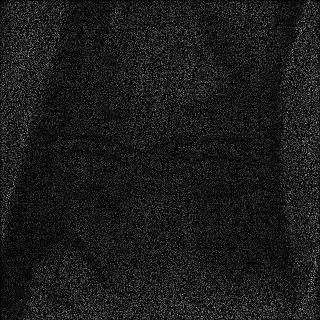
\includegraphics[width=8cm,height=8cm]{../../../regularizers/scripts/gradient/gradient}};

\end{tikzpicture}
\end{document}
